%iffalse
\let\negmedspace\undefined
\let\negthickspace\undefined
\documentclass[journal,12pt,onecolumn]{IEEEtran}
\usepackage[version=4]{mhchem}
\usepackage{chemformula} % for \ch if needed
\usepackage{chemfig}
\usepackage{chemmacros}
\chemsetup{modules = reactions} % Enables reaction arrows
\usepackage{graphicx}
\graphicspath{ {./images/} }

\usepackage{fancyhdr}
\usepackage{geometry}
\usepackage{lastpage}
\usepackage{cite}
\usepackage{amsmath,amssymb,amsfonts,amsthm}
\usepackage{enumitem,multicol}
\usepackage{algorithmic}
\usepackage{graphicx}
\usepackage{textcomp}
\usepackage{xcolor}
\usepackage{txfonts}
\usepackage{listings}
\usepackage{enumitem}
\usepackage{mathtools}
\usepackage{gensymb}
\usepackage{comment}
\usepackage[breaklinks=true]{hyperref}
\usepackage{tkz-euclide} 
\usepackage{listings}
\usepackage{gvv}                                        
%\def\inputGnumericTable{}                                 
                               
\usepackage{color}                                            
\usepackage{array}                                            
\usepackage{longtable}                                       
\usepackage{calc}                                             
\usepackage{multirow}                                         
\usepackage{hhline}                                           
\usepackage{ifthen}                                           
\usepackage{lscape}
\usepackage{tabularx}
\usepackage{array}
\usepackage{float}


\newtheorem{theorem}{Theorem}[section]
\newtheorem{problem}{Problem}
\newtheorem{proposition}{Proposition}[section]
\newtheorem{lemma}{Lemma}[section]
\newtheorem{corollary}[theorem]{Corollary}
\newtheorem{example}{Example}[section]
\newtheorem{definition}[problem]{Definition}
\newcommand{\BEQA}{\begin{eqnarray}}
\newcommand{\EEQA}{\end{eqnarray}}
\newcommand{\define}{\stackrel{\triangle}{=}}
\theoremstyle{remark}

\usepackage[utf8]{inputenc}  

\geometry{margin=1 in}

% Marks the beginning of the document
\begin{document}
\title{
ASSIGNMENT 1: GATE 2007 \\
CY: Chemistry}
\author{AI25BTECH11021 - Abhiram Reddy N}
\maketitle



\begin{enumerate}
  



\item The rate of sulphonation of benzene can be significantly enhanced by the use of
\hfill{\brak{\textbf{GATE CY 2007}}}
\begin{enumerate}
     \item   a mixture of HNO$_3$ and H$_2$SO$_4$
     \item   conc. H$_2$SO$_4$
     \item   a solution of SO$_3$ in H$_2$SO$_4$
     \item   SO$_3$
\end{enumerate}

\item
\schemestart
\chemfig{*6(=-=-=-)} 
\+ 2Na \+ 2\ce{C2H5OH}
\arrow{->[\text{Liq. NH3}]}
\chemfig{*6(--=--=)} 
\+ 2\ce{C2H5ONa}
\schemestop
\\is an example of \hfill{\brak{\textbf{GATE CY 2007}}}

\begin{enumerate}
     \item   Birch reduction
     \item   Clemmenson reduction
     \item   Wolff-Kishner reduction
     \item   Hydride reduction
\end{enumerate}

\item
The major product (X) of the monobromination reaction is
 \hfill{\brak{\textbf{GATE CY 2007}}}

\[
\chemfig{CH_3-[:0]*6(------)} \xrightarrow{\ce{NBS}} \text{(X)}
\]
\begin{multicols}{2}
    
\begin{enumerate}
   \item   \chemfig{Br-CH_2-[:0]-*6(------)}
   \item   \chemfig{CH_3-[:0]*6(---(-Br)---)}
 \item   \chemfig{*6(--((-Br))-((-CH_3))---)}
   \item   \chemfig{*6(-(-[:30](-Br)-[:-30](CH_3))-----)}
  
\end{enumerate}

\end{multicols}

\item  Benzene can not be iodinated with I2 directly. However, in presence of oxidants such as HNO3, iodination is possible. The electrophile formed in this case is
\hfill{\brak{\textbf{GATE CY 2007}}}

\begin{multicols}{4}
    
\begin{enumerate}
   \item   \[
  \left[ \ce{I^+} \right]
  \]
   \item   \[
  \left[ \ce{I^-} \right]
  \]
 \item   \[
  \left[ \ce{^{\delta+}I \cdots ^{\delta+}OH2} \right]^+
  \]

   \item   \[
  \left[ \ce{^{\delta+}I \cdots ^{\delta-}OH2} \right]^+
  \]
  
\end{enumerate}

\end{multicols}

\item Classification of species as Electrophiles (E) and Nucleophiles (N)\hfill{\brak{\textbf{GATE CY 2007}}}

Given species: \ce{SO3}, \ce{Cl^+}, \ce{CH3NH2}, \ce{H3O^+}, \ce{BH3}, \ce{CN^-} 
 


\begin{enumerate}
   
\item  E = \ce{SO3}, \ce{Cl^+}, \ce{BH3} \quad ; \quad N = \ce{CH3NH2}, \ce{H3O^+}, \ce{CN^-} \\
\item  E = \ce{Cl^+}, \ce{H3O^+} \quad ; \quad N = \ce{SO3}, \ce{CH3NH2}, \ce{BH3}, \ce{CN^-} \\
\item  E = \ce{Cl^+}, \ce{H3O^+}, \ce{BH3} \quad ; \quad N = \ce{SO3}, \ce{CH3NH2}, \ce{H3O^+}, \ce{CN^-} \\
\item  E = \ce{SO3}, \ce{Cl^+}, \ce{H3O^+}, \ce{BH3} \quad ; \quad N = \ce{CH3NH2}, \ce{CN^-}
\end{enumerate}

\item The major product obtained upon treatment of compound X with \ce{H2SO4} at 80\degree C is \hfill{\brak{\textbf{GATE CY 2007}}}

  

\textbf{(X)}

\[
\chemfig{CH_3-[:30]CH_2-[:30]C(-[:90]CH_3)(-[:330]OH)-[:30]CH_2-[:30]CH_3}
\]

 

\begin{multicols}{2}
\noindent
\textbf{(A)} \\
\chemfig{CH_3-[:30]CH_2-[:30]CH=[:30]CH-[:30]CH_2-[:30]CH_3}

  

\noindent
\textbf{(B)} \\
\chemfig{CH_3-[:30]C(-[:90]CH_3)-[:330]*5(-----)}

  

\noindent
\textbf{(C)} \\
\chemfig{CH_2=[:30]C(-[:90]CH_3)-[:330]CH_2-[:30]CH_3}

  

\noindent
\textbf{(D)} \\
\chemfig{CH_3-[:30]CH=[:30]C(-[:90]CH_3)-[:330]CH_2-[:30]CH_3}

\end{multicols}

\item \ce{BaTi[Si3O9]} is a class of \hfill{\brak{\textbf{GATE CY 2007}}}
\begin{multicols}{4}
    

\begin{enumerate}
     \item   ortho silicate
     \item   cyclic silicate
     \item   chain silicate
     \item   sheet silicate
\end{enumerate}
\end{multicols}
 

\item The ground state term for \ce{V^{3+}} ion is \hfill{\brak{\textbf{GATE CY 2007}}}
\begin{multicols}{4}
\begin{enumerate}
     \item   $^3F$
     \item   $^2F$
     \item   $^3P$
     \item   $^2D$
\end{enumerate}
\end{multicols}
 

\item In photosynthesis, the predominant metal present in the reaction centre of photosystem II is \hfill{\brak{\textbf{GATE CY 2007}}}
\begin{multicols}{4}
    

\begin{enumerate}
     \item   Zn
     \item   Cu
     \item   Mn
     \item   Fe
\end{enumerate}
\end{multicols}
 

\item The octahedral complex / complex ion which shows both facial and meridional isomers is \hfill{\brak{\textbf{GATE CY 2007}}}
\begin{multicols}{2}
    
\begin{enumerate}
     \item   Triglycinatocobalt(III)
     \item   Tris(ethylenediamine)cobalt(III)
     \item   Dichlorodiglycinatocobalt(III)
     \item   Trioxalatocobaltate(III)
\end{enumerate}
\end{multicols}
 

\item Zn in carbonic anhydrase is coordinated by three histidine and one water molecule. The reaction of \ce{CO2} with this enzyme is an example of \hfill{\brak{\textbf{GATE CY 2007}}}
\begin{multicols}{4}
    

\begin{enumerate}
     \item   electrophilic addition
     \item   electron transfer
     \item   nucleophilic addition
     \item   electrophilic substitution
\end{enumerate}

\end{multicols}
 

\item The difference in the measured and calculated magnetic moment (based on spin-orbit coupling) is observed for \hfill{\brak{\textbf{GATE CY 2007}}}
\begin{multicols}{2}
\begin{enumerate}[leftmargin=*,labelsep=1em]
     \item   Pm$^{3+}$
     \item   Eu$^{3+}$
     \item   Dy$^{3+}$
     \item   Lu$^{3+}$
\end{enumerate}
\end{multicols}
  

\item For a redox reaction, \ce{Cd^{2+} + 2e^- -> Cd}, the \ce{E_{p,\ anodic}} observed in cyclic voltammetry at hanging mercury drop electrode is --650 mV vs. SCE. The expected value for \ce{(E_{p})_{cathodic}} is \hfill{\brak{\textbf{GATE CY 2007}}}
\begin{multicols}{2}
\begin{enumerate}[leftmargin=*,labelsep=1em]
     \item   --708 mV
     \item   --679 mV
     \item   --650 mV
     \item   --621 mV
\end{enumerate}
\end{multicols}
  

\item The dimension of Planck constant is (M, L and T denote mass, length and time respectively) \hfill{\brak{\textbf{GATE CY 2007}}}
\begin{multicols}{2}
\begin{enumerate}[leftmargin=*,labelsep=1em]
     \item   ML$^2$T$^{-2}$
     \item   ML$^2$T$^{-1}$
     \item   M$^2$L$^{-1}$T$^{-1}$
     \item   M$^{-1}$L$^2$T$^{-2}$
\end{enumerate}
\end{multicols}
  

\item For a homonuclear diatomic molecule, the bonding molecular orbital is \hfill{\brak{\textbf{GATE CY 2007}}}
\begin{multicols}{2}
\begin{enumerate}[leftmargin=*,labelsep=1em]
     \item   $\sigma_u$ of lowest energy
     \item   $\sigma_u$ of second lowest energy
     \item   $\pi_g$ of lowest energy
     \item   $\pi_u$ of lowest energy
\end{enumerate}
\end{multicols}
  

\item The selection rules for the appearance of P branch in the rotational-vibrational absorption spectra of a diatomic molecule within rigid rotor-harmonic oscillator model are \hfill{\brak{\textbf{GATE CY 2007}}}
\begin{multicols}{2}
\begin{enumerate}[leftmargin=*,labelsep=1em]
     \item   $\Delta \nu = \pm 1$ and $\Delta J = \pm 1$
     \item   $\Delta \nu = +1$ and $\Delta J = +1$
     \item   $\Delta \nu = +1$ and $\Delta J = -1$
     \item   $\Delta \nu = -1$ and $\Delta J = -1$
\end{enumerate}
\end{multicols}
 

\item The S$_2$ operation on a molecule with the axis of rotation as the z axis, moves a nucleus at (x, y, z) to \hfill{\brak{\textbf{GATE CY 2007}}}
\begin{multicols}{2}
\begin{enumerate}[leftmargin=*,labelsep=1em]
     \item   (-x, -y, z)
     \item   (x, -y, -z)
     \item   (-x, y, -z)
     \item   (-x, -y, -z)
\end{enumerate}
\end{multicols}
 

\item The expression which represents the chemical potential of the $i^{\text{th}}$ species ($\mu_i$) in a mixture ($i \ne j$) is \hfill{\brak{\textbf{GATE CY 2007}}}
\begin{multicols}{2}
\begin{enumerate}[leftmargin=*,labelsep=1em]
     \item   $\left( \frac{\partial E}{\partial n_i} \right)_{S,V,n_j}$
     \item   $\left( \frac{\partial H}{\partial n_i} \right)_{S,P,n_j}$
     \item   $\left( \frac{\partial A}{\partial n_i} \right)_{T,V,n_j}$
     \item   $\left( \frac{\partial G}{\partial n_i} \right)_{T,P,n_j}$
\end{enumerate}
\end{multicols}
 

\item Which of the following statements is \textbf{NOT} correct for a catalyst? \hfill{\brak{\textbf{GATE CY 2007}}}
\begin{multicols}{2}
\begin{enumerate}[leftmargin=*,labelsep=1em]
     \item   It increases the rate of a reaction
     \item   It is not consumed in the course of a reaction
     \item   It provides an alternate pathway for the reaction
     \item   It increases the activation energy of the reaction
\end{enumerate}
\end{multicols}
  

\item The value of the rate constant for the gas phase reaction \ch{2NO2 + F2 -> 2NO2F} is 38 dm$^{3}$ mol$^{-1}$ s$^{-1}$ at 300K. The order of the reaction is \hfill{\brak{\textbf{GATE CY 2007}}}
\begin{multicols}{2}
\begin{enumerate}[leftmargin=*,labelsep=1em]
     \item   0
     \item   1
     \item   2
     \item   3
\end{enumerate}
\end{multicols}

\item Boric acid in aqueous solution in presence of glycerol behaves as a strong acid due to the formation of \hfill{\brak{\textbf{GATE CY 2007}}}
\begin{multicols}{2}
\begin{enumerate}[leftmargin=*,labelsep=1em]
     \item   an anionic metal-chelate
     \item   borate anion
     \item   glycerate ion
     \item   a charge transfer complex
\end{enumerate}
\end{multicols}
  

\item Match the compounds in \textbf{List I} with the corresponding structure / property given in \textbf{List II} \hfill{\brak{\textbf{GATE CY 2007}}}

\begin{tabbing}
\hspace{3cm} \= \textbf{List I} \hspace{5cm} \= \textbf{List II} 

\\
(a) (Ph$_3$P)$_3$RhCl \> (i) Spinel \\
(b) LiCl$_6$ \> (ii) Intercalation \\
(c) PtF$_6$ \> (iii) Oxidising agent \\
(d) Ni$_3$S$_4$ \> (iv) Catalyst for alkane hydrogenation \\

\end{tabbing}


\begin{enumerate}[leftmargin=*,labelsep=1em]
     \item   a - iii \quad b - i \quad c - ii \quad d - iv
     \item   a - iv \quad b - ii \quad c - iii \quad d - i
     \item   a - iii \quad b - ii \quad c - ii \quad d - iv
     \item   a - iv \quad b - iii \quad c - ii \quad d - i
\end{enumerate}

  

\item \ch{W(CO)6} reacts with MeLi to give an intermediate which upon treatment with \ch{CH2N2} gives a compound \textbf{X}. \textbf{X} is represented as \hfill{\brak{\textbf{GATE CY 2007}}}
\begin{multicols}{2}
\begin{enumerate}[leftmargin=*,labelsep=1em]
     \item   WMe$_6$
     \item   (CO)$_5$W-Me
     \item   (CO)$_5$W=C(Me)OMe
     \item   (CO)$_5$W = CMe
\end{enumerate}
\end{multicols}
  

\item Considering the quadrupolar nature of M-M bond in \ch{[Re2Cl8]^{2-}}, the M-M bond order in \ch{[Re2Cl4(PMe2Ph)4]^{+}} and \ch{[Re2Cl4(PMe2Ph)4]} respectively are \hfill{\brak{\textbf{GATE CY 2007}}}
\begin{multicols}{2}
\begin{enumerate}[leftmargin=*,labelsep=1em]
     \item   3.0 and 3.0
     \item   3.0 and 3.5
     \item   3.5 and 3.5
     \item   3.5 and 3.0
\end{enumerate}
\end{multicols}
  

\item A student recorded a polarogram of 2.0 mM Cd$^{2+}$ solution and forgot to add KCl solution. What type of error do you expect in his results? \hfill{\brak{\textbf{GATE CY 2007}}}
\begin{multicols}{2}
\begin{enumerate}[leftmargin=*,labelsep=1em]
     \item   Only migration current will be observed
     \item   Only diffusion current will be observed
     \item   Both migration current as well as diffusion current will be observed
     \item   Both catalytic current as well as diffusion current will be observed
\end{enumerate}
\end{multicols}
  

\item The separation of trivalent lanthanide ions, Lu$^{3+}$, Yb$^{3+}$, Dy$^{3+}$, Eu$^{3+}$ can be effectively done by a cation exchange resin using ammonium \textit{o}-hydroxy isobutyrate as the eluent. The order in which the ions will be separated is \hfill{\brak{\textbf{GATE CY 2007}}}
\begin{multicols}{2}
\begin{enumerate}[leftmargin=*,labelsep=1em]
     \item   Lu$^{3+}$, Yb$^{3+}$, Dy$^{3+}$, Eu$^{3+}$
     \item   Eu$^{3+}$, Dy$^{3+}$, Yb$^{3+}$, Lu$^{3+}$
     \item   Dy$^{3+}$, Yb$^{3+}$, Eu$^{3+}$, Lu$^{3+}$
     \item   Yb$^{3+}$, Dy$^{3+}$, Lu$^{3+}$, Eu$^{3+}$
\end{enumerate}
\end{multicols}
  

\item Arrange the following metal complexes in order of their increasing hydration energy \hfill{\brak{\textbf{GATE CY 2007}}}

\begin{center}
\begin{tabular}{cccc}
\ch{[Mn(H2O)6]^{2+}}$_P$ & \ch{[V(H2O)6]^{2+}}$_Q$ & \ch{[Ni(H2O)6]^{2+}}$_R$ & \ch{[Ti(H2O)6]^{2+}}$_S$
\end{tabular}
\end{center}

\begin{multicols}{2}
\begin{enumerate}[leftmargin=*,labelsep=1em]
     \item   $P < S < Q < R$
     \item   $P < Q < R < S$
     \item   $Q < P < R < S$
     \item   $S < R < Q < P$
\end{enumerate}
\end{multicols}
  

\item In the complex, [Ni$_2$(n$^5$-Cp)$_2$(CO)$_2$], the IR stretching frequency appears at 1857 cm$^{-1}$ (strong) and 1897 cm$^{-1}$ (weak). The valence electron count and the nature of the M-CO bond respectively are \hfill{\brak{\textbf{GATE CY 2007}}}
\begin{multicols}{2}
\begin{enumerate}[leftmargin=*,labelsep=1em]
     \item   16 e$^-$, bridging
     \item   17 e$^-$, bridging
     \item   18 e$^-$, terminal
     \item   18 e$^-$, bridging
\end{enumerate}
\end{multicols}
  

\item The correct classification of [B$_5$H$_5$]$^{2-}$, B$_5$H$_9$ and B$_5$H$_{11}$ respectively is \hfill{\brak{\textbf{GATE CY 2007}}}
\begin{multicols}{2}
\begin{enumerate}[leftmargin=*,labelsep=1em]
     \item   closo, arachno, nido
     \item   arachno, closo, nido
     \item   closo, nido, arachno
     \item   nido, arachno, closo
\end{enumerate}
\end{multicols}
  


\item The compounds \textbf{X} and \textbf{Y} in the following reaction are
\hfill{\brak{\textbf{GATE CY 2007}}}

\[
\chemfig P_4S_{10} \xrightarrow{\ce{EtOH}} \text{(X)}
\xrightarrow{\ce{Cl_2}} \text{(Y)}
 \xrightarrow{\ce{p-O_2NC_6H_4ONa}} \text{Paration} 
\]


\begin{multicols}{2}
\begin{enumerate}[leftmargin=*, labelsep=1em]
     \item   $X = (\mathrm{Et})_2\mathrm{P}(S)SH \quad ; \quad Y = (\mathrm{Et})_2\mathrm{P}(S)Cl$
     \item   $X = (\mathrm{EtO})_2\mathrm{P}(S)SH \quad ; \quad Y = (\mathrm{EtO})_2\mathrm{P}(S)Cl$
     \item   $X = (\mathrm{EtO})_2\mathrm{PSH} \quad ; \quad Y = (\mathrm{EtO})_2\mathrm{PCl}$
     \item   $X = (\mathrm{Et})_3\mathrm{PO} \quad ; \quad Y = (\mathrm{Et})_3\mathrm{PCl}$
\end{enumerate}
\end{multicols}
 

\item Consider the reactions \hfill{\brak{\textbf{GATE CY 2007}}}

\begin{enumerate}
\item \([Cr(H_2O)_6]^{2+} + [CoCl(NH_3)_5]^{2+} \rightarrow [Co(NH_3)_5(H_2O)]^{3+} + [CrCl(H_2O)_5]^{2+}\)
\item \([Fe(CN)_6]^{4-} + [Mo(CN)_8]^{3-} \rightarrow [Fe(CN)_6]^{3-} + [Mo(CN)_8]^{4-}\)
\end{enumerate}

Which one of the following is the correct statement?  

\begin{multicols}{2}
\begin{enumerate} 
 \item   Both involve an inner sphere mechanism  
 \item   Both involve an outer sphere mechanism  
 
 \item   Reaction 1 follows outer sphere and reaction 2 follows inner sphere mechanism  
 \item   Reaction 1 follows inner sphere and reaction 2 follows outer sphere mechanism  
\end{enumerate}
\end{multicols}
  

\item The pair of compounds having the same hybridization for the central atom is  \hfill{\brak{\textbf{GATE CY 2007}}}

\begin{center}
    

\begin{multicols}{2}
\begin{enumerate} 
 \item   XeF$_4$ and [SiF$_6$]$^{2-}$  
 \item   [NiCl$_4$]$^{2-}$ and [PtCl$_4$]$^{2-}$  
 \item   Ni(CO)$_4$ and XeO$_2$F$_2$  
 \item   [Co(NH$_3$)$_6$]$^{3+}$ and [Co(H$_2$O)$_6$]$^{3+}$  
\end{enumerate}
\end{multicols}

\end{center}


\item In the reaction shown below, X and Y respectively are  \hfill{\brak{\textbf{GATE CY 2007}}}

\[
\text{Mn}_2(\text{CO})_{10} \xrightarrow{\text{Na}} (X) \xrightarrow{\text{CH}_3\text{COCl}} (Y)
\]

\begin{multicols}{2}
\begin{enumerate} 
 \item   [Mn(CO)$_4$]$^{2-}$ , [CH$_3$C(O)Mn(CO)$_5$]$^{-}$  
 \item   [Mn(CO)$_5$]$^{-}$ , CH$_3$C(O)Mn(CO)$_5$  
 \item   [Mn(CO)$_5$]$^{-}$ , C1Mn(CO)$_5$  
 \item   [Mn(CO)$_4$]$^{2-}$ , C1Mn(CO)$_5$  
\end{enumerate}
\end{multicols}
  

\item The Lewis acid character of BF$_3$, BCl$_3$ and BBr$_3$ follows the order  \hfill{\brak{\textbf{GATE CY 2007}}}

\begin{multicols}{2}
\begin{enumerate} 
\item BF$_3$ < BBr$_3$ < BCl$_3$  
\item BCl$_3$ < BBr$_3$ < BF$_3$  
\item BF$_3$ < BCl$_3$ < BBr$_3$  
\item BBr$_3$ < BCl$_3$ < BF$_3$  
\end{enumerate}
\end{multicols}
  

\item The compound which shows L$\leftarrow$M charge transfer is  \hfill{\brak{\textbf{GATE CY 2007}}}

\begin{multicols}{2}
\begin{enumerate} 
\item Ni(CO)$_4$  
\item K$_2$Cr$_2$O$_7$  
\item HgO  
 \item   [Ni(H$_2$O)$_6$]$^{2+}$  
\end{enumerate}
\end{multicols}
  

\item The reaction of [PtCl$_4$]$^{2-}$ with NH$_3$ gives rise to  \hfill{\brak{\textbf{GATE CY 2007}}}

\begin{multicols}{2}
\begin{enumerate} 
 \item   [PtCl$_2$(NH$_3$)$_2$]$^{2-}$  
 \item   trans-[PtCl$_2$(NH$_3$)$_2$]  
 \item   [PtCl$_2$(NH$_3$)$_4$]  
 \item   cis-[PtCl$_2$(NH$_3$)$_2$]  
\end{enumerate}
\end{multicols}
  

\item  Zeise's salt is represented as  \hfill{\brak{\textbf{GATE CY 2007}}}

\begin{multicols}{2}
\begin{enumerate} 
 \item   H$_2$PtCl$_6$  
 \item   [PtCl$_4$]$^{2-}$  
 \item   [ZnCl$_4$]$^{2-}$  
 \item   [PtCl$_3$($\eta^2$-C$_2$H$_4$)]$^{-}$  
\end{enumerate}
\end{multicols}
  

\item  The catalyst used in the conversion of ethylene to acetaldehyde using Wacker process is  \hfill{\brak{\textbf{GATE CY 2007}}}

\begin{multicols}{2}
\begin{enumerate} 
\item H$_2$Co(CO)$_4$  
\item PdCl$_4^{2-}$  
\item V$_2$O$_5$  
\item TiCl$_4$ in presence of Al(C$_2$H$_5$)$_3$  
\end{enumerate}
\end{multicols}
  

\item  The temperature of 54 g of water is raised from 15°C to 75°C at constant pressure. The change in the enthalpy of the system (given that $C_{p,m}$ of water = 75 J K$^{-1}$ mol$^{-1}$) is \hfill{\brak{\textbf{GATE CY 2007}}}

\begin{multicols}{2}
\begin{enumerate}
 \item   4.5 kJ
 \item   13.5 kJ
 \item   9.0 kJ
 \item   18.0 kJ
\end{enumerate}
\end{multicols}
  

\item  The specific volume of liquid water is 1.0001 mL g$^{-1}$ and that of ice is 1.0907 mL g$^{-1}$ at 0°C. If the heat of fusion of ice at this temperature is 333.88 J g$^{-1}$, the rate of change of melting point of ice with pressure in deg atm$^{-1}$ will be \hfill{\brak{\textbf{GATE CY 2007}}}

\begin{multicols}{2}
\begin{enumerate}
 \item   $-$0.0075
 \item   0.0075
 \item   0.075
 \item   $-$0.075
\end{enumerate}
\end{multicols}
  

\item  Given that $E^\circ$(Fe$^{3+}$, Fe$^{2+}$) = $-$0.04 V and $E^\circ$(Fe$^{2+}$, Fe) = $-$0.44 V, the value of $E^\circ$(Fe$^{3+}$, Fe) is \hfill{\brak{\textbf{GATE CY 2007}}}

\begin{multicols}{2}
\begin{enumerate}
 \item   0.76 V
 \item   $-$0.40 V
 \item   $-$0.76 V
 \item   0.40 V
\end{enumerate}
\end{multicols}
  

\item  For the reaction P + Q + R $\rightarrow$ S, experimental data for the measured initial rates is given below \hfill{\brak{\textbf{GATE CY 2007}}}

\begin{center}
\begin{tabular}{|c|c|c|c|c|}
\hline
Expt. & Initial conc. P (M) & Initial conc. Q (M) & Initial conc. R (M) & Initial rate (M s$^{-1}$) \\
\hline
1 & 0.2 & 0.5 & 0.4 & $8.0 \times 10^{-3}$ \\
2 & 0.4 & 0.5 & 0.4 & $3.2 \times 10^{-2}$ \\
3 & 0.4 & 0.25 & 0.4 & $1.28 \times 10^{-2}$ \\
4 & 0.1 & 0.25 & 1.6 & $4.0 \times 10^{-3}$ \\
\hline
\end{tabular}
\end{center}

The order of the reaction with respect to P, Q and R respectively is

\begin{multicols}{2}
\begin{enumerate}
 \item   2, 2, 1
 \item   2, 1, 2
 \item   2, 1, 1
 \item   1, 1, 2
\end{enumerate}
\end{multicols}
  

\item  Sucrose is converted to a mixture of glucose and fructose in a pseudo first order process under alkaline conditions. The reaction has a half life of 28.4 min. The time required for the reduction of a 8.0 mM sample of sucrose to 1.0 mM is \hfill{\brak{\textbf{GATE CY 2007}}}

\begin{multicols}{2}
\begin{enumerate}
 \item   56.8 min
 \item   170.4 min
 \item   85.2 min
 \item   227.2 min
\end{enumerate}
\end{multicols}
  

\item  The reaction \hfill{\brak{\textbf{GATE CY 2007}}}
\[
\text{2NO(g)} + \text{O}_2(g) \rightarrow \text{2NO}_2(g)
\]
proceeds via the following steps \hfill{   }
\[
\begin{aligned}
\text{NO + NO} &\xrightarrow{\ce{K_a}} \text{N}_2\text{O}_2 \\
\text{N}_2\text{O}_2 &\xrightarrow{\ce{K_{a'}}} \text{NO + NO} \\
\text{N}_2\text{O}_2 + \text{O}_2 &\xrightarrow{k_b} \text{NO}_2 + \text{NO}_2
\end{aligned}
\]
The rate of this reaction is equal to \hfill{   }
\begin{multicols}{2}
\begin{enumerate} 
    \item $2k_b[\text{NO}]^2[\text{O}_2]$
    \item $\frac{2k_a k_b[\text{NO}]^2[\text{O}_2]}{(k_{-f}+k_b[\text{O}_2])}$
    \item $2k_b[\text{NO}]^2[\text{O}_2]$
    \item $k_b[\text{NO}]^2[\text{O}_2]$
\end{enumerate}
\end{multicols}

\item  40 millimoles of NaOH are added to 100 mL of a 1.2 M HA and Y M NaA buffer resulting in a solution of pH 5.30. Assuming that the volume of the buffer remains unchanged, the pH of the buffer ($K_\text{HA} = 1.00 \times 10^{-5}$) is\hfill{\brak{\textbf{GATE CY 2007}}}
\begin{multicols}{4}
\begin{enumerate} 
    \item 5.30
    \item 5.00
    \item 0.30
    \item 10.30
\end{enumerate}
\end{multicols}

\item  The entropy of mixing of 10 moles of helium and 10 moles of oxygen at constant temperature and pressure, assuming both to be ideal gases, is\hfill{\brak{\textbf{GATE CY 2007}}}
\begin{multicols}{2}
\begin{enumerate} 
    \item 115.3 J K$^{-1}$
    \item 5.8 J K$^{-1}$
    \item 382.9 J K$^{-1}$
    \item 230.6 J K$^{-1}$
\end{enumerate}
\end{multicols}

\item  The ionisation potential of hydrogen atom is 13.6 eV. The first ionisation potential of a sodium atom, assuming that the energy of its outer electron can be represented by a H-atom like model with an effective nuclear charge of 1.84, is\hfill{\brak{\textbf{GATE CY 2007}}}
\begin{multicols}{2}
\begin{enumerate} 
    \item 46.0 eV
    \item 11.5 eV
    \item 5.1 eV
    \item 2.9 eV
\end{enumerate}
\end{multicols}

\item  The quantum state of a particle moving in a circular path in a plane is given by
\[
\Psi_{m}(\phi) = (1/\sqrt{2\pi})e^{im\phi}, m=0,\pm1,\pm2,...
\]
When a perturbation $H_1 = P \cos \phi$ is applied ($P$ is a constant), what will be the first order correction to the energy of the $m^\text{th}$ state\hfill{\brak{\textbf{GATE CY 2007}}}
\begin{multicols}{2}
\begin{enumerate} 
    \item 0
    \item $P(2\pi)$
    \item $P(4\pi)$
    \item $Pm^2(4\pi^2)$
\end{enumerate}
\end{multicols}
  

 \item  The correct statement(s) among the following is/are \\
(i) The vibrational energy levels of a real diatomic molecule are equally spaced. \\
(ii) At 500k, the reaction A $\xrightarrow[ ]{ }$ B is spontaneous when $\Delta $H = 18.83 kj mol$^{-1}$ and $\Delta $S  = 41.84 J K$^{-1}$ mol$^{-1}$. \\
(iii) The process of fluorescence involves transition from a singlet electronic state to another singlet electronic state by absorption of light. \\
(iv) When a constant P is added to each of the possible energies of a system, its entropy remains unchanged. \\
\hfill{\brak{\textbf{GATE CY 2007}}}
\begin{multicols}{2}
\begin{enumerate} 
    \item only i
    \item only ii
    \item both i and iii
    \item both ii and iv
\end{enumerate}
\end{multicols}

\item  Assuming H$_2$ and HD molecules having equal bond lengths, the ratio of the rotational partition functions of these molecules, at temperatures above 100K is \hfill{\brak{\textbf{GATE CY 2007}}}
\begin{multicols}{2}
\begin{enumerate} 
    \item 3/8
    \item 3/4
    \item 1/2
    \item 2/3
\end{enumerate}
\end{multicols}

\item  N noninteracting molecules are distributed among three nondegenerate energy levels $\varepsilon_0 = 0$, $\varepsilon_1 = 1.38 \times 10^{-21}$ J and $\varepsilon_2 = 2.76 \times 10^{-21}$ J at 100K. If the average total energy of the system at this temperature is $1.38 \times 10^{-18}$ J, the number of molecules in the system is \hfill{\brak{\textbf{GATE CY 2007}}}
\begin{multicols}{2}
\begin{enumerate} 
    \item 1000
    \item 1503
    \item 2354
    \item 2987
\end{enumerate}
\end{multicols} 
   

\item  The $J = 0 \rightarrow 1$ rotational transition for $^{1}H^{2}D^{+}$ occurs at 500.72 GHz. Assuming the molecule to be a rigid rotor, the $J = 3 \rightarrow 4$ transition occurs at \hfill{\brak{\textbf{GATE CY 2007}}}
\begin{multicols}{2}
\begin{enumerate} 
    \item 50.1 cm$^{-1}$
    \item 66.8 cm$^{-1}$
    \item 16.7 cm$^{-1}$
    \item 83.5 cm$^{-1}$
\end{enumerate}
\end{multicols}


\item  The rate constants of two reactions at temperature T are $k_1(T)$ and $k_2(T)$ and the corresponding activation energies are $E_1$ and $E_2$ with $E_2 > E_1$. When temperature is raised from $T_1$ to $T_2$, which one of the following relations is correct? \hfill{\brak{\textbf{GATE CY 2007}}}
\begin{multicols}{2}
\begin{enumerate} 
    \item $\dfrac{k_1(T_2)}{k_1(T_1)} > \dfrac{k_2(T_2)}{k_2(T_1)}$
    \item $\dfrac{k_2(T_2)}{k_2(T_1)} > \dfrac{k_1(T_2)}{k_1(T_1)}$
    \item $\dfrac{k_2(T_1)}{k_2(T_2)} > \dfrac{k_1(T_2)}{k_1(T_1)}$
    \item $\dfrac{k_1(T_1)}{k_1(T_2)} > \dfrac{k_2(T_1)}{k_2(T_2)}$
\end{enumerate}
\end{multicols}

\item  The number of degrees of freedom for a system consisting of NaCl(s), Na$^+$(aq) and Cl$^-$(aq) at equilibrium is \hfill{\brak{\textbf{GATE CY 2007}}}
\begin{multicols}{2}
\begin{enumerate} 
    \item 2
    \item 3
    \item 4
    \item 5
\end{enumerate}
\end{multicols} 


\item  Match the structures in \textbf{List I} with their correct names given in \textbf{List II} \hfill{\brak{\textbf{GATE CY 2007}}}

  

\begin{tabular}{m{0.5\textwidth} m{0.5\textwidth}}
\textbf{List I} & \textbf{List II} \\[10pt]

% (a) 2-methyl furan
(a) \quad
\chemfig{*5(-O-=(-CH_3)-=-)}\hspace{0.3cm}  
& 
(i) 2-methyl furan \\[15pt]

% (b) Imidazole
(b) \quad
\chemfig{*5(=N-=-N--)} 
&
(ii) Imidazole \\[15pt]

% (c) 5-hydroxybenzothiazole
(c) \quad
\chemfig{*6((-NH_2)=N-=-=-)} 
&
(iii) 5-hydroxybenzothiazole \\[15pt]

% (d) 2-amino piperidine
(d) \quad
\chemfig{*6((-NH_2)-=-=-=--)} 
&
(iv) 2-amino piperidine \\[15pt]

% (e) 2-amino morpholine
(e) \quad
\chemfig{*6(--(-NH_2)-NH---)} 
&
(v) 2-amino morpholine \\
\end{tabular}

  

\noindent Options:

\begin{multicols}{2}
\begin{enumerate}
    \item a-vii, b-ii, c-vi, d-iii, e-iv
    \item a-vii, b-ii, c-vi, d-viii, e-iv
    \item a-vii, b-ii, c-vi, d-iii, e-v
    \item a-i, b-ii, c-vi, d-iii, e-iv
\end{enumerate}
\end{multicols} 
   

\item  The result of the reduction of either (R) or (S) 2-methylcyclohexanone, in separate reactions, using LiAlH\textsubscript{4} is that the reduction of \hfill{\brak{\textbf{GATE CY 2007}}}

  

\begin{multicols}{2}
\begin{enumerate}
    \item the R enantiomer is stereoselective
    \item the R enantiomer is stereospecific
    \item the S enantiomer is stereospecific
    \item both the R and S enantiomers is stereoselective
\end{enumerate}
\end{multicols}

  


\item  The increasing order of basicity among the following is \hfill{\brak{\textbf{GATE CY 2007}}}

\begin{figure}
    \centering
    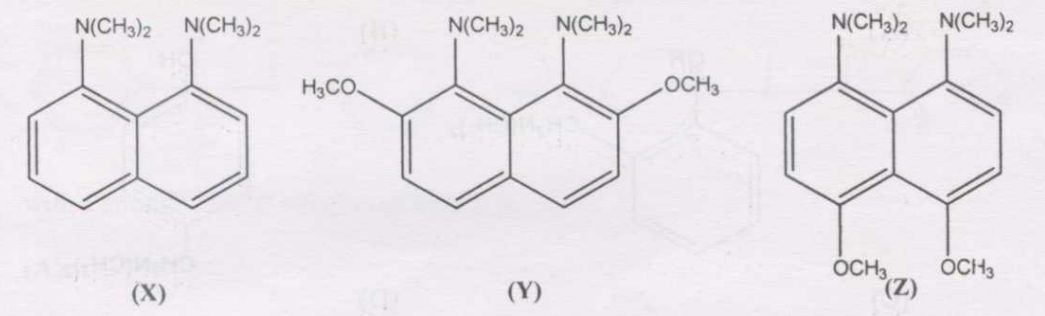
\includegraphics[width=0.5\columnwidth]{figs/image1.png}
    \caption{}
    \label{fig:image1}
\end{figure}



\begin{multicols}{2}
\begin{enumerate}
     \item   Y < X < Z
     \item   Y < Z < X
     \item   X < Z < Y
     \item   X < Y < Z
\end{enumerate}
\end{multicols}

  

\item  In the reaction \hfill{\brak{\textbf{GATE CY 2007}}}

\begin{figure}
    \centering
   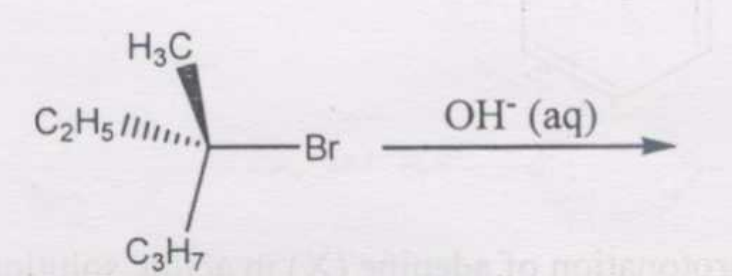
\includegraphics[width=0.5\columnwidth]{figs/image2.png}
    \caption{Caption}
    \label{fig:figure2}
\end{figure}


If the concentration of both the reactants is doubled, then the rate of the reaction will

\begin{multicols}{2}
\begin{enumerate}
     \item   remain unchanged
     \item   quadruple
     \item   reduce to one fourth
     \item   double
\end{enumerate}
\end{multicols}

  

\item  Match the structures in \textbf{List I} with the coupling constant [$^1$J] (Hz) given in \textbf{List II} \hfill{\brak{\textbf{GATE CY 2007}}}

\begin{figure}
    \centering
   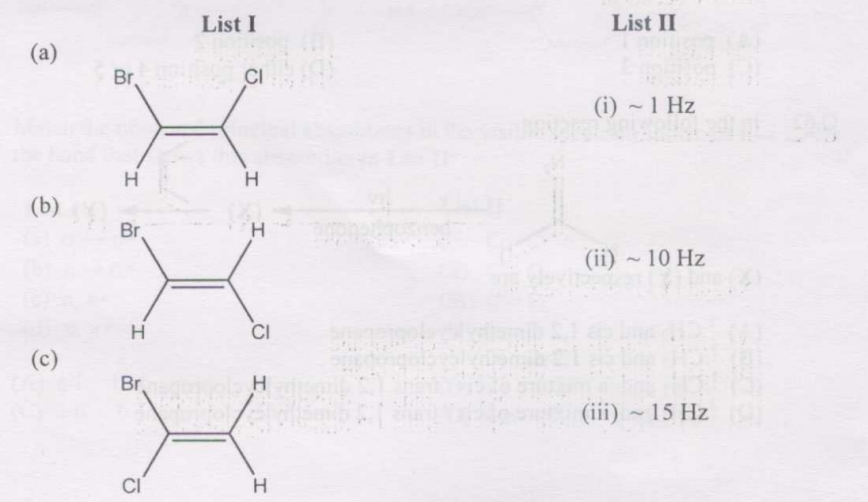
\includegraphics[width=0.5\columnwidth]{figs/image3.png}
    \caption{}
    \label{fig:image3}
\end{figure}


\begin{multicols}{2}
\begin{enumerate}
     \item   a-i \quad b-ii \quad c-iii
     \item   a-ii \quad b-iii \quad c-i
     \item   a-iii \quad b-ii \quad c-i
     \item   a-iii \quad b-i \quad c-ii
\end{enumerate}
\end{multicols}

\item  Phenol on reaction with formaldehyde and dimethyl amine mainly gives \hfill{\brak{\textbf{GATE CY 2007}}}

\begin{figure}
    \centering
   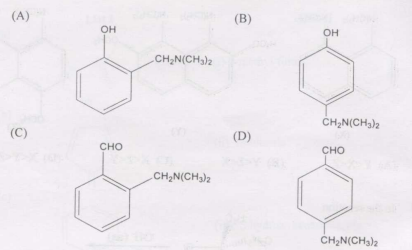
\includegraphics[width=0.5\columnwidth]{figs/image4.png}
    \caption{}
    \label{fig:image4}
\end{figure}


  

\item  The mono protonation of adenine (X) in acidic solution \hfill{\brak{\textbf{GATE CY 2007}}}

\begin{figure}
    \centering
    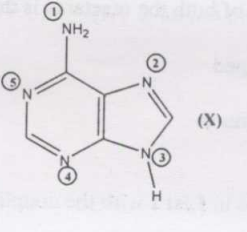
\includegraphics[width=0.5\columnwidth]{figs/image5.png}
    \caption{}
    \label{fig:figure5}
\end{figure}



Mainly occurs at \hfill{  }

\begin{multicols}{2}
\begin{enumerate}
     \item   position 1
     \item   position 2
     \item   position 3
     \item   either position 4 or 5
\end{enumerate}
\end{multicols}

  

\item  In the following reaction \hfill{\brak{\textbf{GATE CY 2007}}}

\begin{figure}
    \centering
    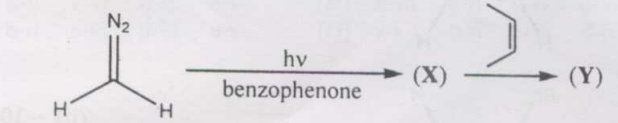
\includegraphics[width=0.5\columnwidth]{figs/image6.png}
    \caption{}
    \label{fig:figure6}
\end{figure}


X and Y respectively are

\begin{multicols}{2}
\begin{enumerate}
     \item   \textsuperscript{1}:CH\textsubscript{2} and cis 1,2 dimethylcyclopropane
     \item   \textsuperscript{3}:CH\textsubscript{2} and cis 1,2 dimethylcyclopropane
     \item   \textsuperscript{1}:CH\textsubscript{2} and a mixture of cis/trans 1,2 dimethylcyclopropane
     \item   \textsuperscript{3}:CH\textsubscript{2} and a mixture of cis/trans 1,2 dimethylcyclopropane
\end{enumerate}
\end{multicols}

\item  The major products obtained upon treating a mixture of \hfill{\brak{\textbf{GATE CY 2007}}}
\begin{figure}
    \centering
    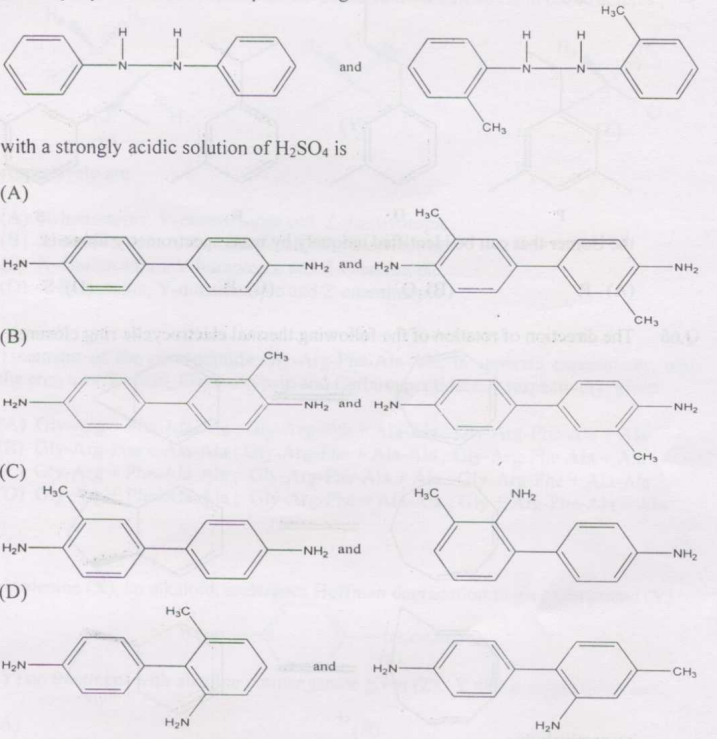
\includegraphics[width=0.5\columnwidth]{figs/image7.png} 
    \caption{}
    \label{fig:figure7}
\end{figure}

   

\item  Match the observed principal absorptions in the visible spectrum shown in \textbf{List I} with the bond that shows this absorption in \textbf{List II} \hfill{\brak{\textbf{GATE CY 2007}}}

\begin{center}
\begin{tabular}{c@{\hspace{3cm}}c}
\textbf{List I} & \textbf{List II} \\
(a) $\sigma \rightarrow \sigma^*$ & (i) C -- C \\
(b) $n \rightarrow \sigma^*$ & (ii) C -- O \\
(c) $n, \pi^*$ & (iii) C = O \\
(d) $\pi, \pi^*$ & (iv) C = C \\
\end{tabular}
\end{center}

\begin{multicols}{2}
\begin{enumerate}
     \item   a-i \quad b-ii \quad c-iii \quad d-iv
     \item   a-i \quad b-iii \quad c-ii \quad d-iv
     \item   a-ii \quad b-i \quad c-iv \quad d-iii
     \item   a-iv \quad b-ii \quad c-iii \quad d-i
\end{enumerate}
\end{multicols}
   

\item  The direction of rotation of the following thermal electrocyclic ring closures respectively is \hfill{\brak{\textbf{GATE CY 2007}}}
\begin{figure}
    \centering
    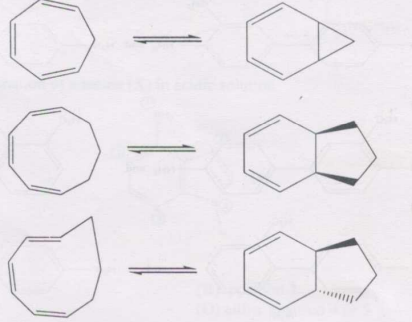
\includegraphics[width=0.5\columnwidth]{figs/image8.png}
    \caption{}
    \label{fig:figure8}
\end{figure}



\begin{multicols}{2}
\begin{enumerate}
     \item   disrotatory, disrotatory, disrotatory
     \item   conrotatory, conrotatory, conrotatory
     \item   disrotatory, disrotatory, conrotatory
     \item   disrotatory, conrotatory, disrotatory
\end{enumerate}
\end{multicols}

  


\item  The molecule(s) that exist as \textit{meso} structure(s) is/are \hfill{\brak{\textbf{GATE CY 2007}}}
\begin{figure}
    \centering
    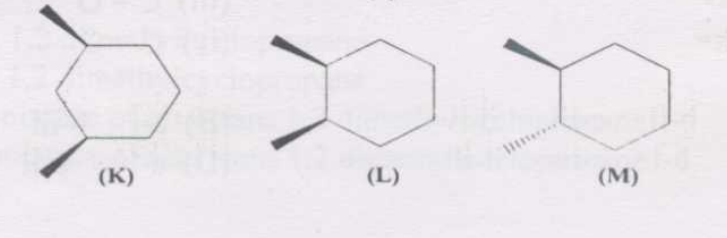
\includegraphics[width=0.5\columnwidth]{figs/image9.png}
    \caption{}
    \label{fig:image9}
\end{figure}




\begin{multicols}{2}
\begin{enumerate}
   \item   only M
   \item   both K and L
   \item   only L
   \item   only K
\end{enumerate}
\end{multicols}

  

\item  The stereochemical descriptors for the atoms labeled H\textsubscript{a} and H\textsubscript{b} in the structures X, Y and Z respectively are \hfill{\brak{\textbf{GATE CY 2007}}}
\begin{figure}
    \centering
    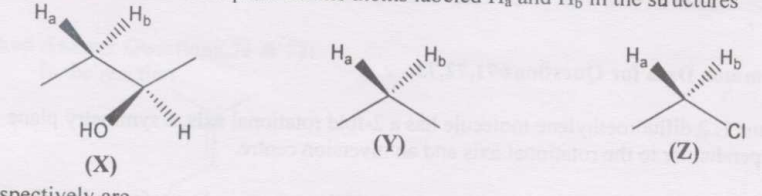
\includegraphics[width=0.5\columnwidth]{figs/image10.png}
    \caption{}
    \label{fig:figure10}
\end{figure}

\begin{multicols}{2}
\begin{enumerate} 
\item X-homotopic, Y-enantiotopic and Z-diastereotopic
\item X-enantiotopic, Y-homotopic and Z-diastereotopic
\item X-diastereotopic, Y-homotopic and Z-enantiotopic
\item X-homotopic, Y-diastereotopic and Z-enantiotopic
\end{enumerate}
\end{multicols}
  

\item  Treatment of the pentapeptide Gly-Arg-Phe-Ala-Ala, in separate experiments, with the enzymes Trypsin, Chymotrypsin and Carboxypeptidase A respectively, gives \hfill{\brak{\textbf{GATE CY 2007}}}

\begin{multicols}{2}
\begin{enumerate} 
\item Gly-Arg + Phe-Ala-Ala ; Gly-Arg-Phe + Ala-Ala ; Gly-Arg-Phe-Ala + Ala
\item Gly-Arg-Phe + Ala-Ala ; Gly-Arg-Phe + Ala-Ala ; Gly-Arg-Phe-Ala + Ala
\item Gly-Arg + Phe-Ala-Ala ; Gly-Arg-Phe-Ala + Ala ; Gly-Arg-Phe-Ala-Ala
\item Gly-Arg + Phe-Ala-Ala ; Gly-Arg-Phe + Ala-Ala ; Gly + Arg-Phe-Ala + Ala
\end{enumerate}
\end{multicols}


\item  Hordenine (X), an alkaloid, undergoes Hoffman degradation to give compound (Y). (Y) on treatment with alkaline permanganate gives (Z). Y and Z respectively are \hfill{\brak{\textbf{GATE CY 2007}}}
\begin{figure}
    \centering
    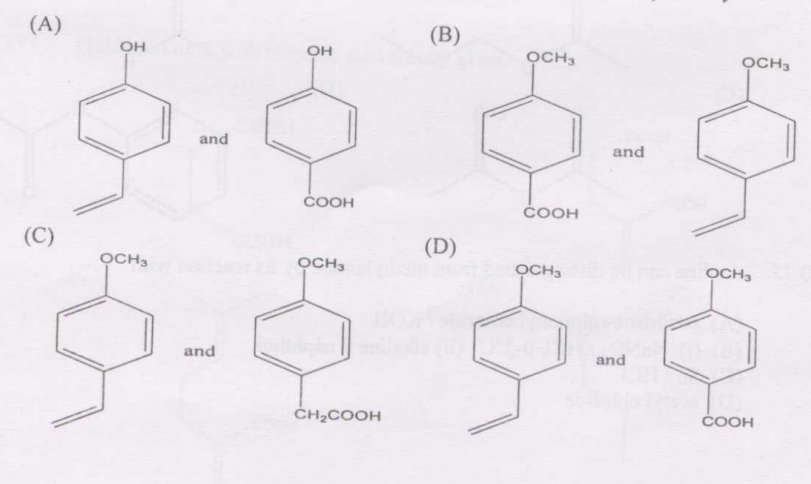
\includegraphics[width=0.5\columnwidth]{figs/image12.png}
    \caption{}
    \label{fig:figure12}
\end{figure}




\item{Common Data for Questions 71, 72, 73:} \\
Trans 1,2 difluoroethylene molecule has a 2-fold rotational axis, a symmetry plane perpendicular to the rotational axis and an inversion centre.

\item  The number of distinct symmetry operations that can be performed on the molecule is \hfill{\brak{\textbf{GATE CY 2007}}}

\begin{multicols}{2}
\begin{enumerate} 
\item 2
\item 4
\item 6
\item 8
\end{enumerate}
\end{multicols}
  

\item  The number of irreducible representations of the point group of the molecule is \hfill{\brak{\textbf{GATE CY 2007}}}

\begin{multicols}{2}
\begin{enumerate} 
\item 1
\item 2
\item 3
\item 4
\end{enumerate}
\end{multicols}
  

\item  When two H atoms of the above molecule are also replaced by F atoms, the point group of the resultant molecule will be \hfill{\brak{\textbf{GATE CY 2007}}}

\begin{multicols}{2}
\begin{enumerate} 
\item C$_i$
\item C$_{2h}$
\item C$_{2v}$
\item D$_{2h}$
\end{enumerate}
\end{multicols}
 

\item{Common Data for Questions 74, 75:} \\
Reactivity of aryl amines towards electrophilic aromatic substitution is much higher than that of aliphatic amines. Hence differential reactivity of the amino group is desirable in many reactions.
  
\item  The compound which on reacting with aniline will \textbf{NOT} form an acetanilide is \hfill{\brak{\textbf{GATE CY 2007}}}
\begin{figure}
    \centering
    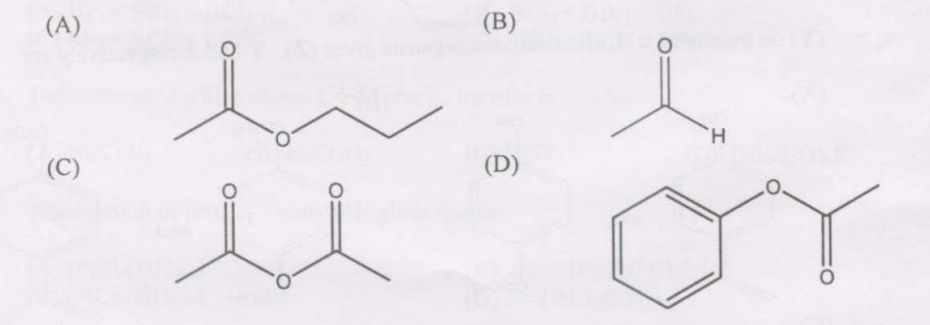
\includegraphics[width=0.5\columnwidth]{figs/image13.png}
    \caption{}
    \label{fig:figure13}
\end{figure}

  

\item  Aniline can be distinguished from methylamine by its reaction with \hfill{\brak{\textbf{GATE CY 2007}}}

\begin{multicols}{2}
\begin{enumerate} 
\item \textit{p}-toluenesulphonyl chloride / KOH
\item (i) NaNO$_2$ / HCl, 0-5$^\circ$C \quad (ii) alkaline $\beta$-naphthol
\item Sn / HCl
\item Acetyl chloride
\end{enumerate}
\end{multicols}

\item{Linked Answer Questions: Q.76 to Q.77 carry two marks each.}

\item  In the reaction \hfill{\brak{\textbf{GATE CY 2007}}}
\begin{figure}
    \centering
    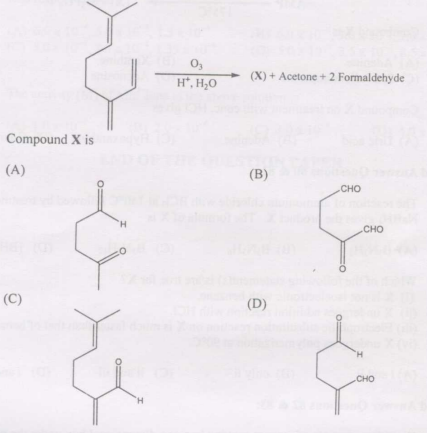
\includegraphics[width=0.5\columnwidth]{figs/image14.png}
    \caption{}
    \label{fig:figure14}
\end{figure}

  

\item  Oxidation of \textbf{X} with chromic acid chiefly gives 
 \hfill{\brak{\textbf{GATE CY 2007}}}
 \begin{figure}
     \centering
     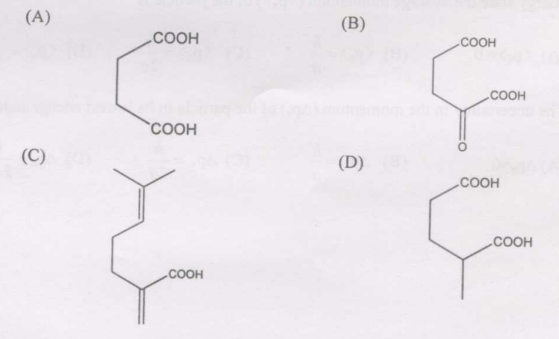
\includegraphics[width=0.5\columnwidth]{figs/image15.png} 
     \caption{}
     \label{fig:figure15}
 \end{figure}
 
   

 \item  In the reaction\\
\hspace*{1cm} AMP \hspace{0.5cm} $\xrightarrow[\text{175°C}]{\text{aq. NH}_3}$ \hspace{0.5cm} (X) + H$_3$PO$_4$\\
Compound X is \hfill{\brak{\textbf{GATE CY 2007}}}
\begin{multicols}{2}
\begin{enumerate} 
    \item Adenine
    \item Xanthine
    \item 2,6-diaminopurine
    \item Adenosine
\end{enumerate}
\end{multicols}
  
\item  Compound X on treatment with conc. HCl gives \hfill{\brak{\textbf{GATE CY 2007}}}
\begin{multicols}{2}
\begin{enumerate} 
    \item Uric acid
    \item Adenine
    \item Hypoxanthine
    \item Guanine
\end{enumerate}
\end{multicols}
  

\item  The reaction of ammonium chloride with BCl$_3$ at 140°C followed by treatment with NaBH$_4$ gives the product X. The formula of X is \hfill{\brak{\textbf{GATE CY 2007}}}
\begin{multicols}{2}
\begin{enumerate} 
    \item B$_3$N$_3$H$_3$
    \item B$_3$N$_3$H$_6$
    \item B$_3$N$_3$H$_{12}$
     \item   [BH-NH]$_n$
\end{enumerate}
\end{multicols}


\item  Which of the following statement(s) is/are true for X?\hfill{\brak{\textbf{GATE CY 2007}}}\\
(i) X is not isoelectronic with benzene.\\
(ii) X undergoes addition reaction with HCl.\\
(iii) Electrophilic substitution reaction on X is much faster than that of benzene.\\
(iv) X undergoes polymerization at 90°C. \hfill{\brak{\textbf{GATE CY 2007}}}
\begin{multicols}{2}
\begin{enumerate} 
    \item i and ii
    \item only ii
    \item ii and iii
    \item i and iv
\end{enumerate}
\end{multicols}


\item  Consider a particle of mass $m$ moving in a one-dimensional box under the potential $V=0$ for $0 \le x \le a$ and $V = \infty$ outside the box. When the particle is in its lowest energy state the average momentum $\langle p_x \rangle$ of the particle is \hfill{\brak{\textbf{GATE CY 2007}}}
\begin{multicols}{2}
\begin{enumerate} 
    \item $\langle p_x \rangle = 0$
    \item $\langle p_x \rangle = \dfrac{h}{a}$
    \item $\langle p_x \rangle = \dfrac{h}{2a}$
    \item $\langle p_x \rangle = \dfrac{h}{2\pi a}$
\end{enumerate}
\end{multicols}


\item  The uncertainty in the momentum ($\Delta p_x$) of the particle in its lowest energy state is \hfill{\brak{\textbf{GATE CY 2007}}}
\begin{multicols}{2}
\begin{enumerate} 
    \item $\Delta p_x = 0$
    \item $\Delta p_x = \dfrac{h}{a}$
    \item $\Delta p_x = \dfrac{h}{2a}$
    \item $\Delta p_x = \dfrac{h}{2\pi a}$
\end{enumerate}
\end{multicols}



\item  In the mixture obtained by mixing 25.0 mL 1.2 $\times$ 10$^{-3}$ M MnCl$_2$ and 35.0 mL of 6.0 $\times$ 10$^{-4}$ M KCl solution, the concentrations (M) of Mn$^{2+}$, K$^+$ and Cl$^-$ ions respectively are \hfill{\brak{\textbf{GATE CY 2007}}}
\begin{multicols}{2}
\begin{enumerate} 
    \item 6.0 $\times$ 10$^{-4}$, 3.0 $\times$ 10$^{-4}$, 1.5 $\times$ 10$^{-3}$
    \item 6.0 $\times$ 10$^{-4}$, 3.0 $\times$ 10$^{-4}$, 9.0 $\times$ 10$^{-4}$
    \item 5.0 $\times$ 10$^{-4}$, 3.5 $\times$ 10$^{-4}$, 1.35 $\times$ 10$^{-3}$
    \item 5.0 $\times$ 10$^{-4}$, 3.5 $\times$ 10$^{-4}$, 8.5 $\times$ 10$^{-4}$
\end{enumerate}
\end{multicols}

\item  The activity (M) of Mn$^{2+}$ ions in the above solution is \hfill{\brak{\textbf{GATE CY 2007}}}
\begin{multicols}{2}
\begin{enumerate} 
    \item 1.0 $\times$ 10$^{-4}$
    \item 2.0 $\times$ 10$^{-4}$
    \item 3.0 $\times$ 10$^{-4}$
    \item 4.0 $\times$ 10$^{-4}$
\end{enumerate}
\end{multicols}

\end{enumerate}
\begin{center}
    \textbf{END OF THE QUESTON PAPER}
\end{center}

\end{document}

